\section{Signal Converter}
The primary purpose of this block is to convert the output from the Torque Sensor to a signal which can be correctly measured by the Control Unit.

\subsection{Design}
The torque-signal and the velocity-signal from the Torque Sensor are measured by the PSoC using different techniques and the Signal Converter must therefore be in charge of three different signal-processing techniques: Rescaling the torque-signal and reduce the noise in the velocity-signal.

\textbf{Rescaling torque-signal}\\
As the PSoC can only measure voltage-levels ranging from $0$ to $+5 V$, and the output-signal from the torque measurement lies between $-5 V$ to $+5 V$, it is necessary to rescale the signal.
\begin{equation}
	V_t = \frac{\tau_{sensor} }{2} + 2.5 V
\end{equation}

\textbf{Noise reduction in velocity-signal}\\
The output-signal for the measured angular velocity lies between the $0$ to $+5 V$ range and can therefore be measured correctly by the PSoC without rescaling. However, the electrical noise in the signal must be reduced, in order to let the PSoC measure correctly.

\subsection{Implementation}
Text

\textbf{Non-inverting adder}\\
Text

\textbf{Noise reduction}\\
The noise reduction is implemented using a 74HC14 hex inverter with Schmitt-trigger inputs. The inverter creates a small propagation delay between the Torque Sensor's output and the PSoC's input. At a 5VDC power supply this delay is given by:\\
$t_{pd} = t_{PHL} = t_{PLH} = 12 ns$


\begin{figure}[H]
	\centering
	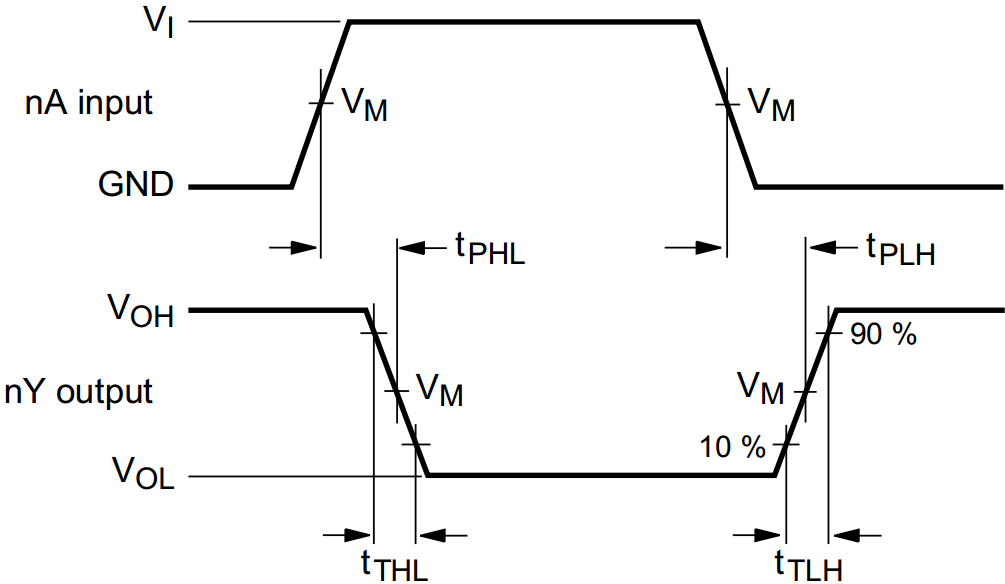
\includegraphics[width=0.5\linewidth]{Hardware/Pictures/74HC14_waveform}
	\caption{Typical inverter-waveform}
	\label{fig:SchmittTrigger_waveform}
\end{figure}

In order to counter the inverting property of 74HC14 the noise reduction must be compromised of two Schmitt-triggers in series. This gives the subsystem a total propagation delay of $24 ns$. As 74HC14 contains six Schmitt-triggers the 4 unused Schmitt-trigger's inputs must be connected to ground in order to prevent unwanted oscilliation.

\subsection{Unity test}
Text